\subsection{Transactions}
\begin{itemize}[label=\(\rhd\)]
    \item \textbf{Transaction}: A logical unit of program execution (i.e., a sequence of actions) that accesses and possibly updates various data items. A transaction is \underline{never executed partially} and it includes one or more DB access operations
    \item For a transaction the following must hold: 
    \begin{itemize}[label=\(\rhd\)]
        \item A transaction must see a consistent database
        \item During transaction execution the DB may be inconsistent
        \item When transaction is committed, the DB must be consistent
    \end{itemize}
    \item Two main issues to deal with:
    \begin{itemize}[label=\(\rhd\)]
        \item Concurrent execution of multiple transactions
        \item Various failures, e.g., hardware failures and system crashes
    \end{itemize}
\end{itemize}

\subsubsection{Transaction States}
\begin{itemize}[label=\(\rhd\)]
    \item \textbf{Active}: (initial state) The transaction stays in this state during execution
    \item \textbf{Partially committed}: After the final statement has been executed
    \item \textbf{Committed}: Transaction has successfully completed and changes are permanent
    \item \textbf{Failed}: After the discovery that normal execution can no longer proceed 
    \item \textbf{Aborted}: After the transaction has been rolled back and the DB restored to its state prior to the start of the transaction. Two possible options after a transaction has been aborted:
    \begin{itemize}[label=\(\rhd\)]
        \item Restart the transaction
        \item Kill the transaction
    \end{itemize}
\end{itemize}

\subsubsection{ACID Properties}
To preserve integrity of data, a transaction must meet the \textbf{ACID} properties:
\begin{itemize}[label=\(\rhd\)]
    \item \textbf{Atomicity}: A transaction's changes to the state are atomic, i.e., either all operations of the transaction are properly reflected in the DB or none are ($\Rightarrow$ recovery manager)
    \item \textbf{Consistency}: A transaction is a correct transformation of a state. The actions (taken as a group) do not violate any of the integrity constraints associated with the state ($\Rightarrow$ application programs and integrity checker)
    \item \textbf{Isolation}: Although multiple transactions may execute concurrently, it appears to each transaction that all other transactions are either executed before or after ($\Rightarrow$ concurrency manager)
    \item \textbf{Durability}: After a transaction completes (commits) successfully, the changes it has made to the database persist, even if there are system failures ($\Rightarrow$ recovery manager)
\end{itemize}

\subsubsection{Schedules}
\begin{itemize}[label=\(\rhd\)]
    \item \textbf{Schedule (or history)}: Sequence of instructions from a set of concurrent transactions that indicate the chronological order in which these instructions are executed
    \begin{itemize}[label=\(\rhd\)]
        \item Must consist of all instructions of all transactions
        \item Must preserve the order of instructions within each individual transaction
    \end{itemize}
    \item \textbf{Serial schedule}: Transactions execute one after the other
    \begin{itemize}[label=\(\rhd\)]
        \item One transaction is completely finished before another transaction starts
        \item Notation: <T1;T3;T2> ("first T1 then T3 then T2)
    \end{itemize}
\end{itemize}

\subsubsection{Serializability}
\begin{itemize}[label=\(\rhd\)]
    \item \textbf{Serializable schedule}: A schedule is serializable if it is equivalent to a serial schedule
    \item There exist different forms of \textbf{schedule equivalence}
\end{itemize}
\bigskip
\textbf{\underline{Conflict Serializability}}\\

\begin{itemize}[label=\(\rhd\)]
    \item Instructions $I_i$ and $I_j$ of transactions $T_i$ and $T_j$, where $T_i \neq T_j$, \textbf{conflict} iff there exists a data item Q accessed by $I_i$ and $I_j$ and at least one of these instructions is a write operation on Q
    \item The goal is to determine \textbf{transformations} of schedules that generate equivalent schedules
    \item Assume a schedule $S$ and two consecutive instructions $I_i$ and $I_{i+1}$ from different transactions. Instructions $I_i$ and $I_{i+1}$ can be \textbf{swapped} if they are \textbf{non-conflicting}, i.e., if
    \begin{itemize}[label=\(\rhd\)]
        \item both are read instructions, or
        \item they refer to different DB items, or
        \item one of them is not a DB operation (i.e., not a read or write)
    \end{itemize}
    \item \textbf{Conflict equivalent schedules}: If a schedule $S$ can be transformed into a schedule $S'$ by a series of non-conflicting swaps of consecutive instructions then $S$ and $S'$ are conflict equivalent
    \item \textbf{Conflict serializable schedule:} A schedule $S$ is conflict serializable iff it is conflict equivalent to a serial schedule 
\end{itemize}

Example: A schedule that is not conflict serializable (unable to swap instructions to obtain the serial schedule <$T_3;T_4$> or <$T_4;T_3$>

\begin{table}[H]
    \centering
    \begin{tabular}{c|c}
        $T_3$ & $T_4$ \\
        \hline
         \textbf{read}(Q) &  \\
         & \textbf{write}(Q) \\
         \textbf{write}(Q) & \\
    \end{tabular}
\end{table}

Example: The following schedule is conflict serializable, since it can be transformed into <$T_1;T_2$> by non-conflicting swaps

\begin{minipage}{0.5\textwidth}
\begin{table}[H]
    \centering
    \begin{tabular}{c|c}
        $T_1$ & $T_2$ \\
        \hline
         \textbf{read}(A) & \\
         \textbf{write}(A) & \\
         & \textbf{read}(A)\\
         & \textbf{write}(A)  \\
         \textbf{read}(B)& \\
        \textbf{write}(B)  & \\
         & \textbf{read}(B) \\
         & \textbf{write}(B) \\
    \end{tabular}
    \caption{Schedule}
\end{table}
\end{minipage}
\begin{minipage}{0.5\textwidth}
    \begin{table}[H]
    \centering
    \begin{tabular}{c|c}
        $T_1$ & $T_2$ \\
        \hline
         \textbf{read}(A) & \\
         \textbf{write}(A) & \\
         \textbf{read}(B)& \\
        \textbf{write}(B)  & \\
         & \textbf{read}(A)\\
         & \textbf{write}(A)  \\
         & \textbf{read}(B) \\
         & \textbf{write}(B) \\
    \end{tabular}
    \caption{Serial schedule}
\end{table}
\end{minipage}

\bigskip
\textbf{\underline{Beyond Conflict Serializability}}\\

\begin{itemize}[label=\(\rhd\)]
    \item A schedule that is not conflict serializable by non-conflicting swaps, may still be equivalent to a serial schedule
    \begin{itemize}[label=\(\rhd\)]
        \item For example due to:
        \begin{itemize}[label=\(\rhd\)]
            \item Blind writes (i.e., write operations without having performed a read operation) 
            \item Or because operations within schedules are commutative 
        \end{itemize}
    \end{itemize}
    \item Determining such equivalence requires to analyse operations other than read and write
\end{itemize}

\bigskip
\textbf{\underline{Testing for Conflict Serializability}}\\

\begin{itemize}[label=\(\rhd\)]
    \item Consider a schedule S of transactions $T_1, T_2, \cdots , T_n$ (we use $r_i(X)$ to denote that transaction $T_i$ reads item X)
    \item \textbf{Precedence graph (conflict graph)}: A directed graph with a node $T_i$ for each transaction and with an edge $T_i \rightarrow T_j$ iff one of the following conditions holds:
    \begin{itemize}[label=\(\rhd\)]
        \item $T_i$ executes write(Q) before $T_j$ executes read(Q)
        \item $T_i$ executes read(Q) before $T_j$ executes write(Q)
        \item $T_i$ executes write(Q) before $T_j$ executes write(Q)
    \end{itemize}
    \item A schedule is \textbf{conflict serializable} if and only if its precedence graph is \textbf{acyclic}
\end{itemize}
Example: A conflict serializable schedule with 5 transactions and precedence graph
\begin{figure}[H]
    \centering
    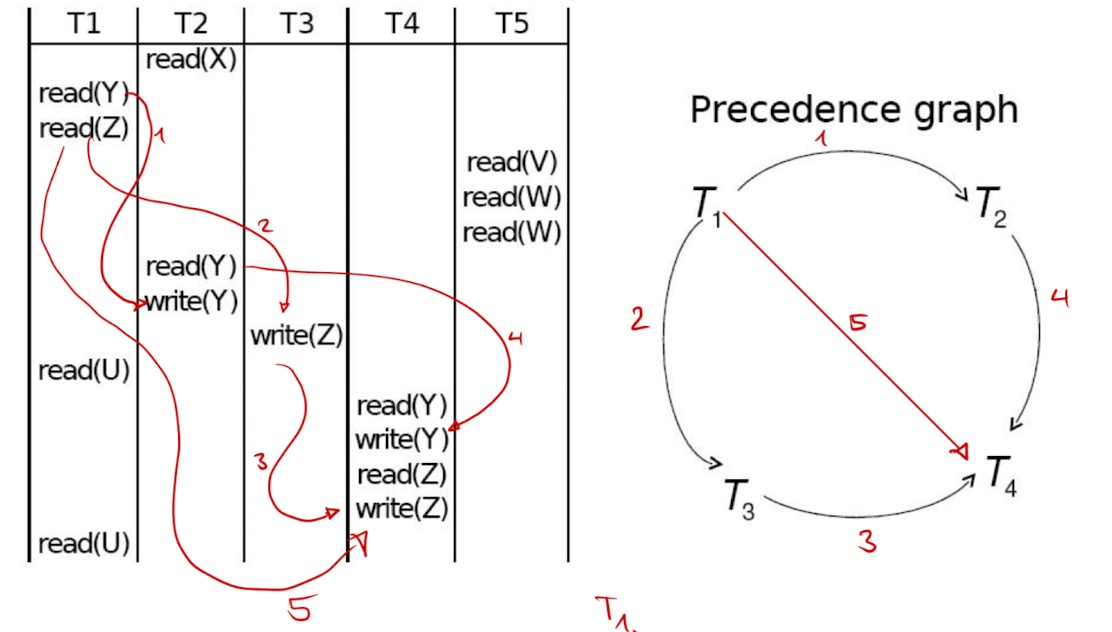
\includegraphics[width=0.5\linewidth]{images/Screenshot 2024-05-25 at 17.55.43.jpg}
    \caption{Topological sorting: $T_5 \rightarrow T_1 \rightarrow T_3 \rightarrow T_2 \rightarrow T_4$}
\end{figure}
\begin{itemize}[label=\(\rhd\)]
    \item Cycle-detection algorithms exist which take $O(n^2)$ time, where $n$ is the \# of vertices in the graph
    \item If the precedence graph is acyclic, the serializability order can be obtained by a topological sorting of the graph. This is a linear order consistent with the partial order of the graph
\end{itemize}

\bigskip
\textbf{\underline{Concurrency Control vs. Serializability Tests}}\\

\begin{itemize}[label=\(\rhd\)]
    \item Testing a schedule for serializability after it has executed is too late
    \item \textbf{Goal}: Develop concurrency control protocols that will assure serializability
    \item \textbf{Concurrency control protocols} will generally not examine the precedence graph as it is being created; instead a \textbf{protocol} will impose a discipline (i.e., a set of rules) that avoids non-serializable schedules
\end{itemize}

\subsubsection{Recoverability}
\begin{itemize}[label=\(\rhd\)]
    \item Need to address the effect of transaction failures on concurrently running transactions
    \item \textbf{Recoverable schedule}: For each pair of transactions $T_i$ and $T_j$ such that $T_j$ reads a data item previously written by $T_i$ the commit operation of $T_i$ must appear before the commit operation of $T_j$
    \item DBMS must ensure that schedules are \textbf{recoverable}
\end{itemize}

\begin{minipage}{0.75\textwidth}
\begin{itemize}[label=\(\rhd\)]
    \item \textbf{Example}: The following schedule s not recoverable if $T_9$ commits immediately after the read operation.
    \begin{itemize}[label=\(\rhd\)]
        \item If $T_8$ aborts, $T_9$ would have read an inconsistent DB state
        \item $T_8$ commits $\Rightarrow T_9$ can commit or abort
        \item $T_8$ aborts $\Rightarrow T_9$ must abort
    \end{itemize}
\end{itemize}
\end{minipage}
\begin{minipage}{0.25\textwidth}
    
    \begin{table}[H]
    \centering
        \begin{tabular}{c|c}
             $T_8$& $T_9$\\
             \hline
             read(A)& \\
             write(A)& \\
             & read(A)\\
             read(B)& \\
        \end{tabular}
    \end{table}
\end{minipage}

\begin{itemize}[label=\(\rhd\)]
    \item \textbf{Cascading rollback}: A single transaction failure leads to a series of transaction rollbacks 
    \begin{itemize}[label=\(\rhd\)]
        \item \textbf{Main problem}: Can lead to the undoing of a significant amount of work (performance issue)
    \end{itemize}
    \item \textbf{Cascade-less schedules}: For each pair of transactions $T_i$ and $T_j$ such that $T_j$ reads a data item previously written by $T_i$, the commit operation of $T_i$ appears before the read operation of $T_j$. This avoids cascading rollbacks. 
    \item Every cascade-less schedule is also recoverable
    \item It is desirable to restrict the schedules to those that are cascade-less
\end{itemize}

\subsection{Concurrency Control}
\subsubsection{Lock-Based Protocols}

\begin{itemize}[label=\(\rhd\)]
    \item One way to \textbf{ensure serializability} is to require that data items be accessed in a mutually exclusive manner, i.e., while one transaction is accessing a data item, no other transaction can modify it
    \item \textbf{Locking}: Mechanism to control concurrent access to a data item
    \item Lock requests are made to concurrency control manager
    \begin{itemize}[label=\(\rhd\)]
        \item Transaction can proceed only after request is granted
    \end{itemize}
    \item Data items can be locked in two modes:
    \begin{itemize}[label=\(\rhd\)]
        \item \textbf{exclusive mode (X)}: Data item can be both read as well as written. X-lock is requested using \textbf{X-lock(A)} instruction
        \item \textbf{shared mode (S)}: Data item can only be read. S-lock is requested using \textbf{S-lock(A)} instruction
    \end{itemize}
    \item Locks can be released: \textbf{U-lock(A)}
    \item \textbf{Locking protocol}: A set of rules followed by all transactions while requesting and releasing locks
\end{itemize}
\begin{minipage}{0.55\textwidth}
\begin{itemize}[label=\(\rhd\)]
    \item \textbf{Lock-compatibility matrix} tells whether two locks are compatible or not.
    \begin{itemize}[label=\(\rhd\)]
        \item Any number of transactions can hold shared locks on a data item.
        \item If any transaction holds an exclusive lock on a data item, no other transaction may hold any lock on that item.
    \end{itemize}
\end{itemize}
\end{minipage}
\hfill
\begin{minipage}{0.4\textwidth}
    \centering
    \begin{tabular}{|c|c|c|c|}
        \hline
        \cellcolor{gray!30} & \multicolumn{2}{c|}{\cellcolor{gray!30}\textbf{lock 2}} \\ \cline{2-3}
        \multirow{-2}{*}{\cellcolor{gray!30}\textbf{lock 1}} & \cellcolor{gray!30}\textbf{S} & \cellcolor{gray!30}\textbf{X} \\ \hline
        \cellcolor{gray!30}\textbf{S} & TRUE & FALSE \\ \hline
        \cellcolor{gray!30}\textbf{X} & FALSE & FALSE \\ \hline
    \end{tabular}
\end{minipage}

\begin{itemize}[label=\(\rhd\)]
    \item \textbf{Locking Rules/Protocol} 
    \begin{itemize}[label=\(\rhd\)]
        \item A transaction may be granted a lock on an item if the requested lock is compatible with locks already held on the item by other transactions
        \item If a lock cannot be granted, the requesting transaction is made to wait until all incompatible locks held by other transactions have been released. The lock is then granted.
    \end{itemize}
\end{itemize}

\subsubsection{Pitfalls of Lock-Based Protocols}

\begin{itemize}[label=\(\rhd\)]
    \item Too early unlocking can lead to non-serializable schedules
    \item Too late unlocking can lead to deadlocks
\end{itemize}

\subsubsection{Two-Phase Locking (2PL)}

\begin{itemize}[label=\(\rhd\)]
    \item \textbf{Two-Phase Locking Protocol}: A locking protocol that ensures conflict-serializable schedules. It works in two phases:
    \begin{itemize}[label=\(\rhd\)]
        \item Phase 1: \textbf{Growing Phase}
        \begin{itemize}[label=\(\rhd\)]
            \item transaction may obtain locks
            \item transaction may not release locks
        \end{itemize}
        \item Phase 2: \textbf{Shrinking Phase}
        \begin{itemize}[label=\(\rhd\)]
            \item transaction may release locks 
            \item transaction may not obtain locks
        \end{itemize}
    \end{itemize}
    \item \textbf{Lock point}: Transition point form phase 1 into phase 2, i.e., when the first lock is released
    \item \textbf{Properties} of the Two-Phase Locking Protocol
    \begin{itemize}[label=\(\rhd\)]
    \item Ensures serializability
    \item Does not ensure freedom from deadlocks
    \item Cascading rollback is possible
\end{itemize}
\item Modifications of the two-phase locking protocol
\begin{itemize}[label=\(\rhd\)]
    \item \textbf{Strict two-phase locking} (S2PL)
    \begin{itemize}[label=\(\rhd\)]
    \item A transaction must hold \textbf{all its exclusive locks} until it commits/aborts
    \item Avoids cascading rollback
\end{itemize}
\item \textbf{Rigorous two-phase locking} (SS2PL)
\begin{itemize}[label=\(\rhd\)]
    \item \textbf{All locks} are held till commit/abort
    \item Transactions can be serialized in the order in which they commit
\end{itemize}
\end{itemize}
\end{itemize}

\subsubsection{Transactions in SQL}
\begin{itemize}[label=\(\rhd\)]
    \item The SQL standard define three \textbf{undesired phenomena} of transactions: 
    \begin{itemize}[label=\(\rhd\)]
        \item \textbf{dirty read}: a transaction sees changes from other uncommitted transactions
        \item \textbf{non-repeatable read}: if a transaction retrieves a row twice it gets different answers
        \item \textbf{phantom reads}: if a transaction retrieves a range of rows twice it retrieves a different answer
    \end{itemize}
    \item The SQL standard uses the undesired phenomena to define four \textbf{isolation levels} as follows: 

\centering
    \begin{tabular}{|c|c|c|c|}
        \hline
         \cellcolor{gray!10}\text{Phenomena} & \cellcolor{gray!10}\text{Dirty read}  & \cellcolor{gray!10}\text{Non-repeatable read} & \cellcolor{gray!10}\text{Phantom read} \\ 
         \hline
       \cellcolor{gray!50}\text{Isolation level} & yes & yes & yes \\ 
       \hline
        \cellcolor{gray!50}\text{read uncommitted} & yes & yes & yes \\ 
        \hline
        \cellcolor{gray!50}\text{read committed} & no & yes & yes \\ 
       \hline
        \cellcolor{gray!50}\text{repeatable read} & no & no & yes \\ 
        \hline
        \cellcolor{gray!50}\text{serializable} & no & no & no \\
        \hline
    \end{tabular}
    
\end{itemize}
\subsubsection{Transactions in DBMSs}

\begin{itemize}[label=\(\rhd\)]
    \item Database systems do not always make \textit{serializable} the default isolation level
    \item The SQL commands \textbf{COMMIT} and \textbf{ROLLBACK} finish the running transaction
\end{itemize}

\subsubsection{Deadlock Handling}

\begin{itemize}[label=\(\rhd\)]
    \item Deadlocks are addressed in two ways: 
    \begin{itemize}[label=\(\rhd\)]
        \item Deadlock prevention protocols are used
        \item Deadlocks are detected and resolved
    \end{itemize}
\end{itemize}

\bigskip
\textbf{\underline{Deadlock Prevention Protocols}}\\

\begin{itemize}[label=\(\rhd\)]
    \item Ensure that the system will never enter into a deadlock state
    \item Two deadlock prevention protocols are \textbf{wait-die} and \textbf{wound-wait}. They use transaction timestamps to prevent deadlocks
    \item With both protocols rolled-back transactions are restarted with their original timestamp. Since older transaction have precedence over newer ones starvation is avoided
    \item Timeout-based protocols can be used to avoid deadlocks:
    \begin{itemize}[label=\(\rhd\)]
        \item A transaction waits for a lock only for a specified amount of time. After that, the wait times out and the transaction is rolled back
        \item Simple to implement; but starvation is possible. Also difficult to determine good value of timeout interval 
    \end{itemize}
\end{itemize}

\bigskip
\textbf{\underline{Deadlock Detection and Recovery}}\\

\begin{itemize}[label=\(\rhd\)]
    \item Deadlocks can be described as a \textbf{wait-for graph}, which consists of a pair $G=(V,E)$,
    \begin{itemize}[label=\(\rhd\)]
        \item V is a set of vertices representing all transactions
        \item E is a set of edges; each element is an ordered pair $T_i\rightarrow T_j$
    \end{itemize}
    \item If $T_i \rightarrow T_j$ is in E, there is a directed edge from $T_i$ to $T_j$, implying that $T_i$ is waiting for $T_j$ to release a data item
    \item If $T_i$ requests a data item being held by $T_j$, edge $T_i \rightarrow T_j$ is inserted in the wait-for graph. This edge is removed when $T_j$ is no longer holding a data item needed by $T_i$
    \item The system is in a deadlock state iff the wait-for graph has a cycle. Must invoke a deadlock-detection algorithm periodically to look for cycles
    \item When a deadlock is detected, the system must \textbf{recover} from the deadlock
    \item The most common solution is to roll back one or more transactions to break the deadlock. Three actions are required: 
    \begin{enumerate}
        \item \textbf{Selection of a victim}: For rollback select the transaction(s) that will incur minimum cost
        \item \textbf{Rollback}: Determine how far to roll back transaction
        \begin{itemize}[label=\(\rhd\)]
            \item Total rollback: Abort the transaction and then restart it
            \item Partial rollback: roll back transaction only as far as necessary to break deadlock
        \end{itemize}
        \item \textbf{Check Starvation}: happens if same transaction is always chosen as victim
        \begin{itemize}[label=\(\rhd\)]
            \item Include the number of rollbacks in the cost factor to avoid starvation
        \end{itemize}
    \end{enumerate}
\end{itemize}

\subsection{Recovery System}
\subsubsection{Log-Based Recovery}
\subsubsection{Deferred DB Modifications}
\subsubsection{Immediate DB Modifications}
\subsubsection{Checkpoints}